\documentclass{article}
\usepackage{fancyhdr}
\usepackage[margin=0.95in]{geometry}
\usepackage{graphicx}
\usepackage{setspace}
\usepackage{indentfirst}
\usepackage{hyperref}
\usepackage{siunitx}
\usepackage{amsmath}
\usepackage{xcolor}
\usepackage[utf8]{inputenc}
\setcounter{tocdepth}{3}
\usepackage{subcaption}
\usepackage{placeins}
\usepackage{float}
\usepackage{listings}
\usepackage{algpseudocode}
\usepackage{enumitem}
\usepackage{algorithm}
\usepackage{mathtools}
\usepackage{amsfonts}
\usepackage{adjustbox}
\usepackage{tikz}
\usetikzlibrary{arrows.meta, calc, positioning}
\usepackage{booktabs}

\colorlet{punct}{red!60!black}
\definecolor{background}{HTML}{EEEEEE}
\definecolor{delim}{RGB}{20,105,176}
\colorlet{numb}{magenta!60!black}

\lstdefinestyle{python}{
    language=Python,
    basicstyle=\ttfamily\small,
    numbers=left,
    numberstyle=\scriptsize,
    stepnumber=1,
    numbersep=8pt,
    showstringspaces=false,
    breaklines=true,
    frame=single,
    backgroundcolor=\color{background},
    keywordstyle=\color{blue!70!black},
    commentstyle=\color{green!40!black},
    stringstyle=\color{orange!60!black}
}

\newcommand{\figplaceholder}[1]{%
  \fbox{\parbox[c][3.4cm][c]{0.88\linewidth}{\centering\small #1}}%
}

\pagestyle{fancy}
\setlength{\arrayrulewidth}{0.5mm}
\setlength{\tabcolsep}{6pt}
\renewcommand{\arraystretch}{1.35}
\setlength{\emergencystretch}{2em}
\hypersetup{
    colorlinks=true,
    linkcolor=blue,
    filecolor=magenta,
    urlcolor=cyan,
    pdftitle={Short-Term Electricity Demand Forecasting for Tetouan City},
    pdfpagemode=FullScreen,
}

\onehalfspacing

\begin{document}

\fancyhead{}
\lhead{Semester 2026.1}
\rhead{Course: Data Science}
\fancyfoot{}
\cfoot{\large Hanoi 2026}
\begin{center}
    \vspace*{0.5cm}
    \begin{Large}
    \textbf{HANOI UNIVERSITY OF SCIENCE AND TECHNOLOGY}

    SCHOOL OF INFORMATION AND COMMUNICATION TECHNOLOGY FACULTY OF COMPUTER SCIENCE
    \end{Large}

    \textbf{--------------------  o0o  ---------------------}

    \vspace{1.0cm}

    
\includegraphics[width=3cm]{figures/hust-logo.png}

    \vspace{0.9cm}

    \begin{huge}
    \textbf{PROJECT REPORT:}
    \end{huge}

    \vspace{0.1cm}

    \begin{Large}
    \textbf{Short-Term Electricity Demand Forecasting\\
    and Peak-Capacity Alerts for Tetouan City}
    \end{Large}
    \rule{\linewidth}{1pt}
    \begin{center}
        \begin{large}
        \textbf{Lecturer: Associate Professor, Ph.D. Than Quang Khuat}\\[0.2cm]
        \textbf{Author:}\\[0.15cm]
        \begin{tabular}{lcl}
            \textbf{Nguyen Phu Luong} & 20261217M & luong.np261217m@sis.hust.edu.vn \\
            \textbf{Ho Xuan Khoa} & 20261257M & khoa.hx261257m@sis.hust.edu.vn \\
            \textbf{Nguyen Tue Lam} & 20261207M & lam.nt261207m@sis.hust.edu.vn \\
        \end{tabular}
        \end{large}
    \end{center}
    \rule{\linewidth}{1pt}

\end{center}

\newpage
\fancyfoot{}
\fancyfoot[C]{\thepage}

\tableofcontents

\newpage
\section*{Abstract}
\addcontentsline{toc}{section}{Abstract}

This report presents a short-term electricity demand forecasting study for
Tetouan, Morocco. The operating problem is to anticipate city load one hour
ahead, and to raise an alert when the forecast crosses a safety capacity
threshold, so that reserve margin can be armed before the evening peak. The
source is the UCI \emph{Power Consumption of Tetouan City} series: 10-minute
measurements from three distribution zones, together with temperature,
humidity, wind speed and diffuse solar radiation. The series is aggregated to
hourly demand. Calendar variables, lagged demand, rolling statistics and
weather features feed a seasonal-naive baseline, a ridge regression, a random
forest, and two gradient-boosting models (XGBoost and LightGBM). Models are
compared on a future test block with MAE, RMSE and WAPE, and peak risk is
scored with peak-magnitude error, peak-timing error and breach anticipation
rate. Square-bracket entries in the result tables are completed from
\path{source_code/outputs/metrics.json} after the pipeline is run.

\noindent\textbf{Keywords:} electricity demand; short-term load forecasting;
time series; gradient boosting; peak capacity; Tetouan.

\section{Introduction and Dataset}
\label{sec:introduction}

\subsection{Problem Statement and Business Understanding}
\label{sec:problem}

Modern cities depend on a distribution network that stays inside its safe
operating range while demand moves with the weather and with daily activity.
In Tetouan the measured load changes through the day and across the year.
A forecast that arrives after the peak has already formed does not help the
operator. The useful forecast is the one issued before the peak, with enough
lead time to commit reserve capacity.

The target of this project is a short-term forecast of city electricity
demand. The primary horizon is the next hour. A 24-hour horizon is a natural
extension and is left as future work in Section~\ref{sec:conclusion}. The
forecast supports two operating decisions:

\begin{enumerate}[label=(\arabic*), itemsep=2pt]
  \item \textbf{Reserve-margin planning.} Compare the forecast with recent
        history and decide how much spare capacity to hold.
  \item \textbf{Peak-capacity alerting.} Raise an alert when the forecast
        exceeds a capacity threshold, so operators can act one to two hours
        before the highest-risk evening window.
\end{enumerate}

The capacity threshold \(\tau\) used in this study is the 95th percentile of
hourly demand on the training block. It is an empirical stand-in for a
published equipment rating. Replacing \(\tau\) with a utility-defined limit
does not change the rest of the pipeline.

\subsection{Primary Dataset Description}
\label{sec:dataset}

The dataset is the open UCI collection \emph{Power Consumption of Tetouan
City} \cite{uci-tetouan, salam2018}. It records 10-minute observations for
calendar year 2017. Each row contains weather measurements and the power of
three distribution zones. Table~\ref{tab:columns} lists the fields used in
this project.

\begin{table}[h]
  \centering
  \small
  \begin{tabular}{@{}llp{7.2cm}@{}}
    \toprule
    Field & Role & Description \\
    \midrule
    DateTime & Index & Timestamp of the 10-minute sample \\
    Temperature & Weather & Ambient temperature (\(^\circ\mathrm{C}\)) \\
    Humidity & Weather & Relative humidity \\
    Wind Speed & Weather & Wind speed \\
    General diffuse flows & Weather & General diffuse solar radiation \\
    Diffuse flows & Weather & Diffuse solar radiation \\
    Zone 1, Zone 2, Zone 3 & Load & Power of the three distribution zones (kW) \\
    \bottomrule
  \end{tabular}
  \caption{Fields retained from the UCI Tetouan series.}
  \label{tab:columns}
\end{table}

City demand at a 10-minute stamp is the sum of the three zones. Forecasting
is performed on an hourly series. Inside each clock hour the pipeline averages
the weather variables and averages city demand. Averaging keeps the target in
kilowatts of mean power. Summing the six raw power readings inside an hour
would inflate the unit and would no longer match a capacity rating expressed
in kW.

After aggregation, the hourly table is the modelling table. The first 168
hours are consumed by the weekly lag, so the supervised sample starts once
\texttt{lag\_168} is defined. Exact row counts, the calendar span, and the
mean load of each zone are recorded in \texttt{outputs/metrics.json} under
\texttt{raw} and \texttt{profile} when \texttt{run\_pipeline.py} is executed.
Fill Table~\ref{tab:dataset-size} from that file.

\begin{table}[h]
  \centering
  \small
  \begin{tabular}{@{}ll@{}}
    \toprule
    Quantity & Value \\
    \midrule
    Raw rows (10-minute) & [XX] \\
    Hourly rows & [XX] \\
    Supervised rows after lag warm-up & [XX] \\
    First timestamp & [YYYY-MM-DD HH:MM] \\
    Last timestamp & [YYYY-MM-DD HH:MM] \\
    Mean city demand & [XX] kW \\
    \bottomrule
  \end{tabular}
  \caption{Dataset size after download and hourly aggregation.}
  \label{tab:dataset-size}
\end{table}

\section{Analytical Methodology}
\label{sec:methodology}

\subsection{Data Preprocessing and Feature Engineering}
\label{sec:features}

Preprocessing is deterministic and uses only information that is available
when the forecast for hour \(t\) is issued. Weather at hour \(t\) is treated
as a forecast the operator already holds. Demand features use hours strictly
before \(t\).

\paragraph{Aggregation.}
\texttt{src/data\_loader.py} downloads the UCI file, parses the timestamp, sums
the three zones into \texttt{total\_kw}, and resamples to one-hour bins.
Weather columns and zone loads are averaged inside the hour.

\paragraph{Calendar features.}
From the timestamp the pipeline builds hour of day (\(0\)--\(23\)), day of
week (\(0\)--\(6\)), month, and a weekend flag \texttt{is\_weekend}. These
variables let a tree model represent the daily and weekly cycle without a
separate seasonal decomposition.

\paragraph{Lag features.}
Demand at \(t-1\,\mathrm{h}\), \(t-2\,\mathrm{h}\), \(t-24\,\mathrm{h}\) and
\(t-168\,\mathrm{h}\) is added so the model can use short-run persistence, the
previous day, and the same hour of the previous week. The weekly lag is also
the forecast of the seasonal-naive baseline.

\paragraph{Rolling-window features.}
A trailing mean and a trailing standard deviation are computed on windows of
3, 6 and 24 hours. Each window is applied to the series shifted by one hour.
The value at time \(t\) therefore does not enter its own features. This is
the leakage control described in Section~\ref{sec:leakage}.

\paragraph{Weather and interaction features.}
Temperature, humidity, wind speed and the two diffuse-radiation channels are
kept as exogenous inputs. Because the link between temperature and load is
curved (cooling load rises once the day is hot), the feature set also
includes a cooling degree above \(22^\circ\mathrm{C}\), squared temperature,
and the product of temperature and hour. Tree ensembles can split on these
terms directly. The linear ridge model receives the same columns after
standardisation, so the comparison stays on one feature matrix.

\subsection{Exploratory Data Analysis}
\label{sec:eda}

Exploration is done on the hourly series before any model is scored on the
test block. Four views are required. Each figure below is a placeholder for
the PNG written by \texttt{src/evaluation.py} into \texttt{outputs/figures/}.
Replace the box with \verb|\includegraphics| once the file exists.

\begin{figure}[h]
  \centering
  \figplaceholder{Line plot: mean demand by hour, weekday and weekend\\
  (\texttt{daily\_profile.png}), plus a two-week trace (\texttt{weekly\_series.png})\\
  and monthly means (\texttt{monthly\_mean.png}).}
  \caption{Demand level across the day, a sample of weeks, and the year.}
  \label{fig:seasonality}
\end{figure}

The daily profile shows when the city peaks. The weekly trace shows the
repeat of that shape from one day to the next. The monthly bars show the
seasonal lift, which in this climate is expected to follow temperature.

\begin{figure}[h]
  \centering
  \figplaceholder{Scatter of temperature against demand (\texttt{temp\_scatter.png})\\
  and the weather correlation heatmap (\texttt{correlation\_heatmap.png}).}
  \caption{Association between weather and city demand.}
  \label{fig:weather}
\end{figure}

The scatter is the check for a non-linear temperature response. The heatmap
ranks linear association of temperature, humidity, wind and radiation with
demand. Record the Pearson correlations from \texttt{profile.corr\_with\_demand}
in the text under the figure after the run. Temperature is the weather
variable the operating discussion relies on.

\begin{figure}[h]
  \centering
  \figplaceholder{Autocorrelation bars for lags 0 to 168 hours\\
  (\texttt{autocorrelation.png}).}
  \caption{Autocorrelation of hourly city demand.}
  \label{fig:acf}
\end{figure}

The autocorrelation plot justifies the lag set. Peaks near 24 hours and
168 hours support the daily and weekly features. The values at lags 1, 2, 24
and 168 are stored in \texttt{profile.acf}.

\subsection{Modeling and Validation Approach}
\label{sec:models}

The supervised table is cut into three contiguous blocks in time order. There
is no shuffle and no overlap. With the default ratios the earliest 70\% is
the training block \(D_{\mathrm{train}}\), the next 15\% is the validation
block \(T_{\mathrm{valid}}\), and the last 15\% is the test block
\(T_{\mathrm{test}}\). Hyperparameters are chosen by validation MAE.
\(T_{\mathrm{test}}\) is scored once, after that choice.

\begin{table}[h]
  \centering
  \small
  \begin{tabular}{@{}llll@{}}
    \toprule
    Block & Role & Rows & Span \\
    \midrule
    \(D_{\mathrm{train}}\) & Fit the model & [XX] & [start] to [end] \\
    \(T_{\mathrm{valid}}\) & Select hyperparameters & [XX] & [start] to [end] \\
    \(T_{\mathrm{test}}\) & Report MAE, RMSE, WAPE, peak scores & [XX] & [start] to [end] \\
    \bottomrule
  \end{tabular}
  \caption{Chronological backtest. Fill the cells from \texttt{metrics.json} key \texttt{splits}.}
  \label{tab:splits}
\end{table}

Five forecasters share that split.

\begin{enumerate}[label=(\arabic*), itemsep=2pt]
  \item \textbf{Seasonal naive.} The forecast for hour \(t\) is the observed
        demand at \(t-168\). This baseline is strong whenever the weekly cycle
        dominates, and it is the reference for every learned model.
  \item \textbf{Ridge regression.} A standardised linear model. The penalty
        \(\alpha\) is chosen from \(\{0.1, 1, 10, 100\}\) on
        \(T_{\mathrm{valid}}\).
  \item \textbf{Random forest} \cite{breiman2001}. Two depths are compared on
        the validation block. The forest captures threshold effects of
        temperature and hour that a single linear coefficient cannot.
  \item \textbf{XGBoost} \cite{chen2016}. Gradient boosting with early
        stopping on \(T_{\mathrm{valid}}\). Learning rate and tree depth are
        selected by validation MAE.
  \item \textbf{LightGBM} \cite{ke2017}. The same protocol as XGBoost, with
        the number of leaves in place of depth. LightGBM is the model used
        for the feature-importance discussion and for the default dashboard
        view.
\end{enumerate}

The selected parameter dictionary for each model is written to
\texttt{selected\_params} in the metrics file. Paste that dictionary into
the appendix or under Table~\ref{tab:scores} when the report is finalised.

\section{Evaluation Results and Insights}
\label{sec:results}

Square-bracket numbers in this section are placeholders. They are replaced
by the fields of \path{source_code/outputs/metrics.json}. The pipeline
does not tune on \(T_{\mathrm{test}}\).

\subsection{Model Performance Evaluation}
\label{sec:performance}

On a test block of \(n\) hours with demand \(y_t\) and forecast
\(\hat{y}_t\), the three error scores are
\begin{align}
  \mathrm{MAE} &= \frac{1}{n}\sum_{t=1}^{n}\lvert y_t-\hat{y}_t\rvert, \label{eq:mae}\\
  \mathrm{RMSE} &= \sqrt{\frac{1}{n}\sum_{t=1}^{n}(y_t-\hat{y}_t)^2}, \label{eq:rmse}\\
  \mathrm{WAPE} &= \frac{\sum_{t=1}^{n}\lvert y_t-\hat{y}_t\rvert}{\sum_{t=1}^{n}\lvert y_t\rvert}. \label{eq:wape}
\end{align}
MAE and RMSE are reported in kW. RMSE penalises large misses more than MAE,
which matters for hours near the capacity limit. WAPE scales the absolute
error by total demand, so it can be read as a system-wide percentage.

\begin{table}[h]
  \centering
  \small
  \begin{tabular}{@{}lrrr@{}}
    \toprule
    Model & MAE (kW) & RMSE (kW) & WAPE (\%) \\
    \midrule
    Seasonal naive & [XX] & [XX] & [XX] \\
    Ridge & [XX] & [XX] & [XX] \\
    Random forest & [XX] & [XX] & [XX] \\
    XGBoost & [XX] & [XX] & [XX] \\
    LightGBM & [XX] & [XX] & [XX] \\
    \bottomrule
  \end{tabular}
  \caption{Test-block scores. Source: \texttt{test\_scores} in \texttt{metrics.json}.}
  \label{tab:scores}
\end{table}

\begin{figure}[h]
  \centering
  \figplaceholder{Bar chart of test MAE and RMSE (\texttt{model\_comparison.png})\\
  and a two-week overlay of actual demand, the best forecast, and \(\tau\)\\
  (\texttt{forecast\_test.png}).}
  \caption{Error comparison and a visual check on the opening of \(T_{\mathrm{test}}\).}
  \label{fig:comparison}
\end{figure}

The improvement of a learned model against the seasonal naive is
\[
  \frac{\mathrm{MAE}_{\mathrm{naive}}-\mathrm{MAE}_{\mathrm{model}}}{\mathrm{MAE}_{\mathrm{naive}}}.
\]
Report that percentage from \texttt{mae\_improvement\_vs\_naive\_pct}. The
discussion should state whether LightGBM or XGBoost reduces both typical
error (MAE, WAPE) and large error (RMSE) relative to the weekly baseline.
A lower MAE alone is not enough if the peak hours remain biased.

\subsection{Peak Capacity and Risk Metrics}
\label{sec:peak}

Average error can look acceptable while the forecast still misses the hour
that threatens the network. Three peak scores are therefore computed on
\(T_{\mathrm{test}}\) only.

\paragraph{Peak magnitude error.}
For each test day, take the actual peak and the forecast peak and record the
absolute gap in kW. The reported value is the mean gap over days that contain
at least 12 hours.

\paragraph{Peak timing error.}
For the same days, record the circular distance in hours between the clock
time of the actual peak and the clock time of the forecast peak. A timing
error of one hour still leaves a short window in which to arm reserve. An
error of several hours does not.

\paragraph{Breach anticipation rate.}
Let \(\tau\) be the training 95th percentile, stored as \texttt{threshold\_kw}
(numeric value [XX] kW). A breach hour is an hour with \(y_t>\tau\). The
breach anticipation rate is the share of those hours for which the forecast
also exceeds \(\tau\):
\begin{equation}
  \mathrm{BAR}
  = \frac{\lvert\{t\in T_{\mathrm{test}}: y_t>\tau \ \mathrm{and}\ \hat{y}_t>\tau\}\rvert}
         {\lvert\{t\in T_{\mathrm{test}}: y_t>\tau\}\rvert}.
  \label{eq:bar}
\end{equation}
The one-hour-ahead forecast is issued before the hour closes, so a hit in
\eqref{eq:bar} is an alert that precedes the realised breach. Alert precision,
the share of threshold crossings that were real, is stored beside BAR so a
high hit rate is not confused with a model that alerts every hour.

\begin{table}[h]
  \centering
  \small
  \begin{tabular}{@{}lrrrr@{}}
    \toprule
    Model & Peak magnitude (kW) & Peak timing (h) & BAR (\%) & Alert precision (\%) \\
    \midrule
    Seasonal naive & [XX] & [XX] & [XX] & [XX] \\
    Ridge & [XX] & [XX] & [XX] & [XX] \\
    Random forest & [XX] & [XX] & [XX] & [XX] \\
    XGBoost & [XX] & [XX] & [XX] & [XX] \\
    LightGBM & [XX] & [XX] & [XX] & [XX] \\
    \bottomrule
  \end{tabular}
  \caption{Peak scores on \(T_{\mathrm{test}}\). Source: \texttt{peak} in \texttt{metrics.json}.}
  \label{tab:peak}
\end{table}

\subsection{Findings and Operating Implications}
\label{sec:insights}

Two exogenous drivers are the focus of the interpretation. Hour of day sets
the shape of the daily cycle. Temperature, together with the cooling-degree
and squared-temperature terms, sets how high that cycle rises on a hot day.
Lag and rolling features will often take a large share of LightGBM gain,
because a one-hour-ahead forecast is strongly autoregressive. The importance
figure should therefore be read in two layers: overall gain, and gain inside
the weather and calendar group. Fill the ranking from
\texttt{lightgbm\_importance} and \texttt{lightgbm\_importance\_groups}.

\begin{figure}[h]
  \centering
  \figplaceholder{Top LightGBM features by gain share (\texttt{feature\_importance.png})\\
  and the share of hours above \(\tau\) by clock hour (\texttt{breach\_by\_hour.png}).}
  \caption{Drivers of the forecast and the clock hours that cross the capacity threshold.}
  \label{fig:importance}
\end{figure}

The breach-by-hour profile is the basis for the reserve rule. Complete the
following statement from \texttt{breach\_rate\_by\_hour\_pct}. The design
target of the study is the evening window from 18:00 to 21:00, which is
expected to concentrate threshold crossings and therefore to need reserve
armed one to two hours earlier. If the measured profile peaks in a
neighbouring window, state that window and keep the same lead time.

\begin{quote}
On the hourly series, the hours from [HH:00] to [HH:00] show the highest
rate of demand above \(\tau\) ([XX]\% of hours in the busiest clock hour).
Reserve for that window should be committed one to two hours in advance.
Temperature and hour of day are the leading exogenous contributors to the
peak. Their LightGBM gain shares are [XX]\% and [XX]\%.
\end{quote}

\section{Main Code Components}
\label{sec:code}

\subsection{Code Base Architecture}
\label{sec:architecture}

All executable code lives under \texttt{source\_code/}. The report and this
chapter only describe that tree. Figure~\ref{fig:pipeline} is the runtime
path from the raw UCI file to the dashboard.

\begin{figure}[h]
  \centering
  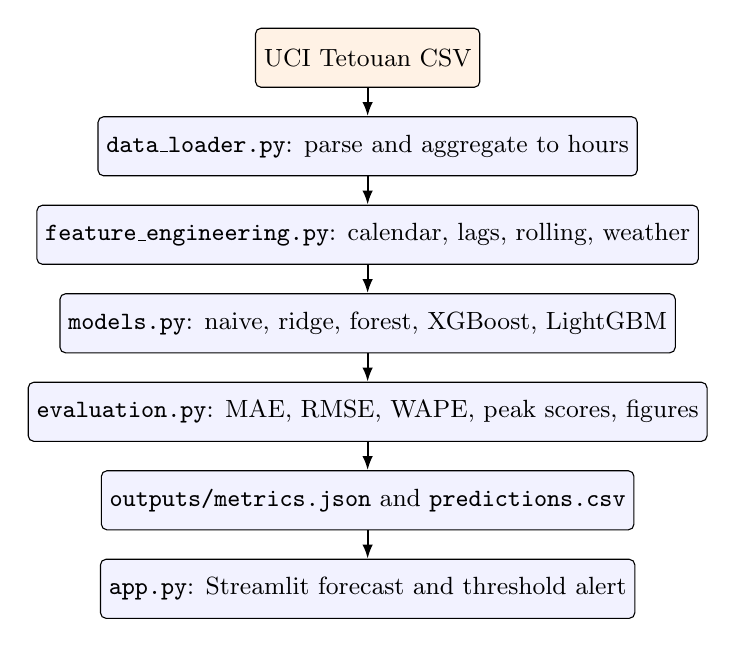
\begin{tikzpicture}[
    node distance=3.6mm,
    box/.style={draw, rounded corners=2pt, fill=blue!5, align=center,
                font=\small, inner sep=3pt, minimum height=7.5mm},
    src/.style={draw, rounded corners=2pt, fill=orange!10, align=center,
                font=\small, inner sep=3pt, minimum height=7.5mm},
    arr/.style={-{Latex[length=1.8mm]}, thick}
  ]
    \node[src] (uci) {UCI Tetouan CSV};
    \node[box, below=of uci] (load) {\texttt{data\_loader.py}: parse and aggregate to hours};
    \node[box, below=of load] (feat) {\texttt{feature\_engineering.py}: calendar, lags, rolling, weather};
    \node[box, below=of feat] (model) {\texttt{models.py}: naive, ridge, forest, XGBoost, LightGBM};
    \node[box, below=of model] (eval) {\texttt{evaluation.py}: MAE, RMSE, WAPE, peak scores, figures};
    \node[box, below=of eval] (out) {\texttt{outputs/metrics.json} and \texttt{predictions.csv}};
    \node[box, below=of out] (app) {\texttt{app.py}: Streamlit forecast and threshold alert};
    \draw[arr] (uci) -- (load);
    \draw[arr] (load) -- (feat);
    \draw[arr] (feat) -- (model);
    \draw[arr] (model) -- (eval);
    \draw[arr] (eval) -- (out);
    \draw[arr] (out) -- (app);
  \end{tikzpicture}
  \caption{Pipeline from the public series to the alert dashboard.}
  \label{fig:pipeline}
\end{figure}

\begin{table}[h]
  \centering
  \small
  \begin{tabular}{@{}lp{9.4cm}@{}}
    \toprule
    Path & Responsibility \\
    \midrule
    \texttt{src/data\_loader.py} & Download the UCI file if it is not cached, standardise column names, sum the three zones, and aggregate to hourly demand. \\
    \texttt{src/feature\_engineering.py} & Build calendar flags, lags, shifted rolling statistics and temperature interactions. Cut the table into \(D_{\mathrm{train}}\), \(T_{\mathrm{valid}}\) and \(T_{\mathrm{test}}\). \\
    \texttt{src/models.py} & Fit the seasonal naive, ridge, random forest, XGBoost and LightGBM models. Choose hyperparameters on the validation block. \\
    \texttt{src/evaluation.py} & Compute MAE, RMSE, WAPE and the peak metrics, and write the figures listed in Sections~\ref{sec:eda} and~\ref{sec:results}. \\
    \texttt{run\_pipeline.py} & Run the four modules and store \texttt{outputs/metrics.json} plus \texttt{outputs/predictions.csv}. \\
    \texttt{app.py} & Streamlit page: test-block forecast, capacity line, breach-anticipation summary and an alert when the forecast exceeds \(\tau\). \\
    \bottomrule
  \end{tabular}
  \caption{Modules in \texttt{source\_code/}.}
  \label{tab:modules}
\end{table}

The dashboard reads saved predictions. It does not retrain. Changing a model
hyperparameter means re-running \texttt{run\_pipeline.py}, then refreshing
the Streamlit page.

\subsection{Tech Stack}
\label{sec:stack}

The language is Python 3.12. Table~\ref{tab:stack} lists the libraries pinned
in \texttt{source\_code/requirements.txt} and the role each one plays.

\begin{table}[h]
  \centering
  \small
  \begin{tabular}{@{}ll@{}}
    \toprule
    Library & Role in this project \\
    \midrule
    \texttt{pandas}, \texttt{numpy} & Tables, resampling, lags and rolling windows \\
    \texttt{scikit-learn} & Ridge, random forest, MAE during model selection \\
    \texttt{xgboost}, \texttt{lightgbm} & Gradient-boosting forecasters \\
    \texttt{matplotlib}, \texttt{seaborn} & EDA figures and the test-set charts \\
    \texttt{streamlit} & Forecast and alert dashboard \\
    \bottomrule
  \end{tabular}
  \caption{Python stack.}
  \label{tab:stack}
\end{table}

No extra service is required. The UCI file is fetched over HTTPS on the first
run and cached under \texttt{source\_code/data/raw/}. Later runs reuse the
cache.

\section{Difficulties and Solutions}
\label{sec:difficulties}

\subsection{Data Leakage in a Time Series}
\label{sec:leakage}

A random row split mixes later hours into the training set. Neighbours of a
test hour then appear on both sides of the split, and lagged copies of the
target leak the answer. The resulting MAE looks strong and does not survive
the next week of operations.

The project uses a blocked temporal split. \(D_{\mathrm{train}}\),
\(T_{\mathrm{valid}}\) and \(T_{\mathrm{test}}\) are contiguous, ordered and
disjoint (Section~\ref{sec:models}). Rolling means and rolling standard
deviations are computed on the demand series after a one-hour shift, so hour
\(t\) is absent from the features that predict it. Validation labels are used
to choose tree size, learning rate and the ridge penalty. They are not used
as training targets, and the test block is not used to pick a model.

\subsection{Non-linear Weather Response}
\label{sec:nonlinear}

A straight line in temperature understates the load on hot afternoons, when
cooling equipment switches on and demand bends upward. Humidity and radiation
move with temperature, so a single coefficient is a poor summary of the
weather effect.

Two complementary fixes are in the feature module and in the model module.
The feature module adds cooling degree, squared temperature and the
temperature-by-hour product, which give the linear model a limited ability to
bend. The tree models (random forest, XGBoost, LightGBM) partition
temperature and hour into regions, so the same hot hour can receive a
different leaf value from a mild hour. The scatter plot in
Figure~\ref{fig:weather} is the diagnostic that this structure is worth
including. The gain shares in Figure~\ref{fig:importance} are the check that
the fitted model actually uses it.

\subsection{Error at the Peak, Hidden by the Mean}
\label{sec:peak-error}

MAE averages every hour. A quiet night with a small error can offset an
evening miss that crosses the capacity threshold. An operator who sees only
MAE will not know whether the peak hour and the peak level were forecast in
time.

The evaluation module therefore scores peaks separately
(Section~\ref{sec:peak}). Peak magnitude error measures the level miss.
Peak timing error measures whether the forecast peak falls on the right hour.
Breach anticipation rate measures whether hours above \(\tau\) were flagged
before they occurred. The dashboard repeats the same threshold on the plotted
forecast, so the numeric BAR and the on-screen alert refer to one rule.

\section{Conclusion and Future Work}
\label{sec:conclusion}

The study specifies a full path from the public Tetouan series to an
operating alert. Ten-minute zone measurements are summed and aggregated to
hourly city demand. Calendar, lag, rolling and weather features are built
without using the future. A seasonal-naive baseline, ridge regression, a
random forest, XGBoost and LightGBM are compared on a later test block that
was not used for training or for model selection. Beside MAE, RMSE and WAPE,
the report records peak magnitude, peak timing and breach anticipation, which
are the scores that speak to reserve-margin decisions.

Once Table~\ref{tab:scores} and Table~\ref{tab:peak} are filled, the
conclusion should state the best model by MAE and whether that same model
also leads on breach anticipation. The operating recommendation follows the
hour profile in Figure~\ref{fig:importance}: arm reserve one to two hours
before the clock window that most often exceeds \(\tau\), with the evening
hours from 18:00 to 21:00 as the window this design is built to protect.

Two extensions stay outside the present pipeline. The first is a quantile
forecast, so the alert can be raised from an upper quantile rather than from
a single point prediction. The second is a multi-horizon forecast at 1 hour,
6 hours and 24 hours, using a separate model or a direct horizon feature for
each lead time. Both extensions reuse the same chronological split and the
same peak metrics.

\addcontentsline{toc}{section}{References}

\begin{thebibliography}{10}

\bibitem{uci-tetouan} D. Dua and C. Graff, ``UCI Machine Learning Repository:
Power Consumption of Tetouan City.'' [Online]. Available:
\url{https://archive.ics.uci.edu/dataset/849/power+consumption+of+tetouan+city}

\bibitem{salam2018} A. Salam and A. El Hibaoui, ``Comparison of Machine
Learning Algorithms for the Power Consumption Prediction: Case Study of
Tetouan city,'' in \emph{Proc. 6th International Renewable and Sustainable
Energy Conference (IRSEC)}, 2018.

\bibitem{hyndman} R. J. Hyndman and G. Athanasopoulos, \emph{Forecasting:
Principles and Practice}, 3rd ed. OTexts, 2021. [Online]. Available:
\url{https://otexts.com/fpp3/}

\bibitem{breiman2001} L. Breiman, ``Random Forests,'' \emph{Machine Learning},
vol. 45, no. 1, pp. 5--32, 2001.

\bibitem{chen2016} T. Chen and C. Guestrin, ``XGBoost: A Scalable Tree
Boosting System,'' in \emph{Proc. 22nd ACM SIGKDD International Conference
on Knowledge Discovery and Data Mining}, 2016, pp. 785--794.

\bibitem{ke2017} G. Ke, Q. Meng, T. Finley, T. Wang, W. Chen, W. Ma, Q. Ye,
and T.-Y. Liu, ``LightGBM: A Highly Efficient Gradient Boosting Decision
Tree,'' in \emph{Advances in Neural Information Processing Systems}, 2017.

\bibitem{sklearn} F. Pedregosa et al., ``Scikit-learn: Machine Learning in
Python,'' \emph{Journal of Machine Learning Research}, vol. 12,
pp. 2825--2830, 2011.

\end{thebibliography}

\appendix

\section{Reproducing the study}
\label{sec:reproduce}

From the repository root, the commands in Listing~\ref{lst:commands} create a
virtual environment, install the stack, fit the models, and open the
dashboard. The first pipeline run downloads the UCI CSV into
\texttt{source\_code/data/raw/}. A second run reuses that file.

\begin{lstlisting}[style=python, caption={Setup, training and dashboard.}, label={lst:commands}]
cd source_code
python -m venv .venv
.venv/Scripts/python -m pip install -r requirements.txt
.venv/Scripts/python run_pipeline.py
.venv/Scripts/python -m streamlit run app.py
\end{lstlisting}

On macOS or Linux, replace \path{.venv/Scripts/python} with
\path{.venv/bin/python}. The pipeline writes:

\begin{itemize}[itemsep=1pt]
  \item \texttt{outputs/metrics.json}, the source for every square-bracket
        number in Chapters~\ref{sec:dataset}, \ref{sec:models} and~\ref{sec:results};
  \item \texttt{outputs/predictions.csv}, the series read by \texttt{app.py};
  \item \texttt{outputs/figures/*.png}, the charts named in the figure boxes.
\end{itemize}

Copy the PNG files into \path{report/figures/} and replace each
\verb|\figplaceholder| with an \verb|\includegraphics| of the matching file.

\section{Compiling the report}

The report is the \texttt{article} source in this folder. From
\texttt{report/}:

\begin{lstlisting}[style=python, caption={Three pdflatex passes.}, label={lst:latex}]
pdflatex -interaction=nonstopmode main
pdflatex -interaction=nonstopmode main
pdflatex -interaction=nonstopmode main
\end{lstlisting}

A shell script with the same passes is \texttt{report/compile.sh}. On
Windows, run \texttt{report/compile.bat}. \texttt{report/compile.ps1} is the
same build, but PowerShell may refuse it when script execution is disabled.
The bibliography is inline (\texttt{thebibliography}), so BibTeX is not required.

\section{Work record}

\begin{table}[h]
  \centering
  \small
  \begin{tabular}{@{}ll@{}}
    \toprule
    Name & Contribution \\
    \midrule
    Luong Nguyen Phu & Pipeline, dashboard and report template \\
    Additional member & Contribution \\
    \bottomrule
  \end{tabular}
  \caption{Division of work. Add rows for the rest of the group.}
  \label{tab:work}
\end{table}


\end{document}
